% !TeX program = xelatex
\documentclass[a4paper,11pt]{article}
\usepackage[a4paper,top=2.45cm,bottom=2.35cm,left=2.65cm,right=2.35cm,headheight=15pt]{geometry}
\usepackage{fontspec,amsmath,amssymb,booktabs,tabularx,array,graphicx,tikz}
\usetikzlibrary{arrows.meta,positioning,shapes.geometric}
\usepackage{xcolor,fancyhdr,titlesec,caption,subcaption,enumitem,hyperref,bookmark,microtype,lastpage,url}
\definecolor{Navy}{HTML}{17365D}\definecolor{Blue}{HTML}{2F75B5}\definecolor{PaleBlue}{HTML}{EAF2F8}\definecolor{Slate}{HTML}{52616B}\definecolor{LightRule}{HTML}{C9D5E2}
\IfFontExistsTF{Times New Roman}{\setmainfont{Times New Roman}}{\setmainfont{Latin Modern Roman}}
\IfFontExistsTF{Arial}{\setsansfont{Arial}}{\setsansfont{Latin Modern Sans}}
\IfFontExistsTF{Menlo}{\setmonofont{Menlo}}{\setmonofont{Latin Modern Mono}}
\hypersetup{colorlinks=true,linkcolor=Navy,urlcolor=Blue,pdfauthor={Hua Yingjie},pdftitle={Experiment 1: Object Detection and Recognition}}
\graphicspath{{figures/}{images/}}
\setlength{\parindent}{1.5em}\setlength{\parskip}{0.18em}
\setlength{\emergencystretch}{1.5em}
\setlist{nosep,leftmargin=2.2em}
\captionsetup{font=small,labelfont={bf,color=Navy},labelsep=quad,skip=6pt}
\titleformat{\section}{\Large\bfseries\sffamily\color{Navy}}{\thesection}{0.75em}{}[\vspace{2pt}\color{LightRule}\titlerule]
\titleformat{\subsection}{\large\bfseries\sffamily\color{Blue}}{\thesubsection}{0.65em}{}
\titleformat{\subsubsection}{\normalsize\bfseries\sffamily\color{Slate}}{\thesubsubsection}{0.55em}{}
\titlespacing*{\section}{0pt}{1.6em}{0.8em}\titlespacing*{\subsection}{0pt}{1.1em}{0.45em}
\pagestyle{fancy}\fancyhf{}
\fancyhead[L]{}
\fancyhead[R]{\small\sffamily\color{Slate}Experiment 1: Object Detection and Recognition}
\fancyfoot[C]{\small\sffamily\color{Slate}\thepage\ / \pageref{LastPage}}
\renewcommand{\headrulewidth}{0.45pt}\renewcommand{\footrulewidth}{0pt}

\begin{document}
\begin{titlepage}\thispagestyle{empty}
\begin{tikzpicture}[remember picture,overlay]
 \fill[white] (current page.south west) rectangle (current page.north east);
 \fill[Navy] (current page.north west)--(current page.north east)--([yshift=-11.7cm]current page.north east)--([yshift=-13.0cm]current page.north west)--cycle;
 \fill[Blue] ([yshift=-12.75cm]current page.north west)--([yshift=-11.55cm]current page.north east)--([yshift=-12.05cm]current page.north east)--([yshift=-13.25cm]current page.north west)--cycle;
 \draw[white,opacity=.10,line width=22pt] ([xshift=-1.0cm,yshift=-3.2cm]current page.north east) circle (3.0cm);
 \draw[white,opacity=.16,line width=1.4pt] ([xshift=-1.0cm,yshift=-3.2cm]current page.north east) circle (1.75cm);
 \draw[white,opacity=.16,line width=1.1pt,rounded corners=7pt] ([xshift=-4.0cm,yshift=-1.65cm]current page.north east) rectangle ([xshift=-0.8cm,yshift=-4.6cm]current page.north east);
 \foreach \a in {0,45,...,315}{\fill[white,opacity=.32] ([xshift=-1.0cm,yshift=-3.2cm]current page.north east) ++(\a:1.75cm) circle (1.4pt);}
 \node[anchor=west,text=white,font=\sffamily\bfseries\fontsize{19}{23}\selectfont] at ([xshift=2.55cm,yshift=-3.25cm]current page.north west){EXPERIMENT 1};
 \draw[white,opacity=.72,line width=1.5pt] ([xshift=2.55cm,yshift=-3.75cm]current page.north west)--([xshift=5.25cm,yshift=-3.75cm]current page.north west);
 \node[anchor=west,text=white,align=left,font=\sffamily\bfseries\fontsize{31}{37}\selectfont] at ([xshift=2.55cm,yshift=-6.0cm]current page.north west){Object Detection\\and Recognition};
 \fill[PaleBlue,rounded corners=5pt] ([xshift=2.55cm,yshift=-16.0cm]current page.north west) rectangle ([xshift=11.0cm,yshift=-20.8cm]current page.north west);
 \fill[Blue] ([xshift=2.55cm,yshift=-16.0cm]current page.north west) rectangle ([xshift=2.68cm,yshift=-20.8cm]current page.north west);
 \node[anchor=west,text=Blue,font=\sffamily\bfseries\large] at ([xshift=3.1cm,yshift=-17.05cm]current page.north west){GROUP 11};
 \node[anchor=west,text=Navy,font=\sffamily\bfseries\LARGE] at ([xshift=3.1cm,yshift=-18.35cm]current page.north west){Hua Yingjie};
 \node[anchor=west,text=Slate,font=\sffamily\large] at ([xshift=3.1cm,yshift=-19.48cm]current page.north west){Student ID \quad 24020036025};
 \foreach \x/\y in {13.1/-17.0,14.0/-17.0,14.9/-17.0,15.8/-17.0,13.1/-17.9,14.0/-17.9,14.9/-17.9,15.8/-17.9,13.1/-18.8,14.0/-18.8,14.9/-18.8,15.8/-18.8}{\fill[Blue!35] ([xshift=\x cm,yshift=\y cm]current page.north west) circle (1.7pt);}
 \draw[Blue!28,line width=1.1pt,rounded corners=4pt] ([xshift=13.55cm,yshift=-19.25cm]current page.north west) rectangle ([xshift=16.25cm,yshift=-21.25cm]current page.north west);
 \draw[Navy!28,line width=1.1pt,rounded corners=4pt] ([xshift=14.25cm,yshift=-20.0cm]current page.north west) rectangle ([xshift=17.0cm,yshift=-22.0cm]current page.north west);
 \node[anchor=south east,text=Navy,font=\sffamily\bfseries\small,align=right] at ([xshift=-2.0cm,yshift=1.65cm]current page.south east){OCEAN UNIVERSITY OF CHINA};
\end{tikzpicture}\mbox{}
\end{titlepage}

\pagenumbering{Roman}\setcounter{page}{1}
\section*{Abstract}\addcontentsline{toc}{section}{Abstract}
This report presents an end-to-end desktop object detection system designed for deployment on an NVIDIA Jetson edge device. The system detects three classes---mouse, keyboard, and cup---and covers data acquisition, automatic pre-annotation, manual review, dataset auditing, YOLOv8 transfer learning, independent evaluation, real-time camera inference, and a ROS2-compatible output interface. The integrated dataset contains approximately 650 source images from self-collected scenes, supplementary online samples, and negative backgrounds. A fully audited core subset contains 225 source images and 687 positive bounding boxes; 15 orphan annotation files were identified and isolated during quality control. Cup-focused offline augmentation adds 45 training samples with geometrically transformed labels, producing a 270-image training representation with 935 boxes, including 116 Cup instances. YOLOv8n was trained for 100 epochs on an Apple Silicon Mac using the PyTorch MPS backend. Validation achieved a precision of 0.806, recall of 0.894, mAP@0.5 of 0.888, and mAP@0.5:0.95 of 0.814. The final Jetson video contains 300 frames at 1280$\times$720 over 20 s. Inspected frames show an on-screen rate of approximately 14.8--15.0 FPS, above the required 5 FPS, and include detections of Keyboard, Mouse, and Cup.

\vspace{0.8em}\noindent\textbf{Keywords:} object detection; YOLOv8; Jetson; automatic pre-annotation; dataset quality audit; edge deployment; ROS2
\clearpage\tableofcontents\clearpage
\pagenumbering{arabic}\setcounter{page}{1}

\section{Objectives and Requirements}
Desktop object detection is a fundamental perception task in robotic manipulation, visual servoing, and human-robot interaction. Unlike an offline benchmark, this experiment requires both model training and deployment on a Jetson platform with a live camera and a processing speed of at least 5 FPS. The work therefore considers data quality, detection accuracy, inference latency, and interface extensibility as one engineering system.

The objectives are to build a three-class dataset, accelerate annotation through human-reviewed pre-annotations, train and evaluate YOLOv8n, deploy the model on Jetson, visualize class labels, boxes and confidence values, and provide structured detection output for ROS2 integration.

\begin{table}[htbp]\centering\caption{Course requirements and corresponding evidence}\label{tab:req}
{\renewcommand{\arraystretch}{1.22}\begin{tabular}{>{\raggedright\arraybackslash}m{4.7cm}>{\raggedright\arraybackslash}m{9.3cm}}\toprule
\textbf{Requirement} & \textbf{Completion and evidence}\\\midrule
At least two desktop-object classes & Three classes: Mouse, Keyboard, and Cup\\
Self-collection, annotation, and training & Multi-source acquisition, pre-annotation, manual review, and YOLOv8 training completed\\
Run recognition on Jetson & Live camera inference completed; see Section~\ref{sec:jetson}\\
Show class, box, and confidence & All three items are overlaid in the recorded output\\
Publish detection results through ROS2 & Publisher and message schema completed; payload validated offline on Mac, while live topic echo remains an on-device integration item\\
Test 20 objects with at least 80\% accuracy & A controlled procedure and record sheet are provided for on-site acceptance\\
At least 5 FPS on Jetson & Recorded interface displays approximately 14.8--15.0 FPS in inspected frames\\
Save results and representative errors & Final video contains a transient extra Keyboard box and an occlusion-related oversized Mouse box\\\bottomrule
\end{tabular}}\end{table}

\section{System Architecture}
The workflow consists of data engineering, model training, edge deployment, and error-driven feedback. The Mac performs data cleaning, splitting, training, and evaluation. The Jetson performs camera capture, inference, visualization, logging, and message publication. Misclassified, missed, or low-confidence frames can be returned to the labeling stage for iterative improvement.

\begin{figure}[htbp]\centering
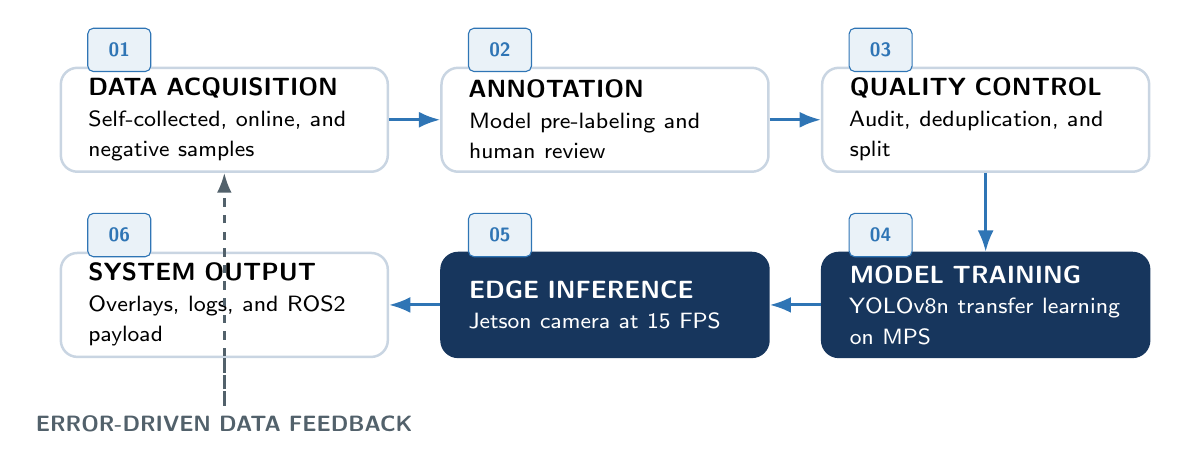
\begin{tikzpicture}[
 stage/.style={rounded corners=6pt,draw=LightRule,line width=0.9pt,fill=white,text width=3.45cm,minimum height=1.32cm,align=left,font=\small\sffamily,inner xsep=10pt},
 active/.style={stage,draw=Navy,fill=Navy,text=white},
 badge/.style={rounded corners=2pt,draw=Blue,fill=PaleBlue,text=Blue,minimum width=8mm,minimum height=5.5mm,inner sep=1pt,font=\scriptsize\sffamily\bfseries},
 arrow/.style={-{Latex[length=2.7mm]},line width=1.05pt,draw=Blue},
 feedback/.style={-{Latex[length=2.5mm]},line width=0.9pt,draw=Slate,dashed}]
 \node[stage](collect){\textbf{DATA ACQUISITION}\\\footnotesize Self-collected, online, and negative samples};
 \node[stage,right=0.65cm of collect](label){\textbf{ANNOTATION}\\\footnotesize Model pre-labeling and human review};
 \node[stage,right=0.65cm of label](audit){\textbf{QUALITY CONTROL}\\\footnotesize Audit, deduplication, and split};
 \node[active,below=1.0cm of audit](train){\textbf{MODEL TRAINING}\\\footnotesize YOLOv8n transfer learning on MPS};
 \node[active,left=0.65cm of train](jetson){\textbf{EDGE INFERENCE}\\\footnotesize Jetson camera at 15 FPS};
 \node[stage,left=0.65cm of jetson](ros){\textbf{SYSTEM OUTPUT}\\\footnotesize Overlays, logs, and ROS2 payload};
 \node[badge,anchor=south west] at ([xshift=10pt,yshift=-2pt]collect.north west){01};
 \node[badge,anchor=south west] at ([xshift=10pt,yshift=-2pt]label.north west){02};
 \node[badge,anchor=south west] at ([xshift=10pt,yshift=-2pt]audit.north west){03};
 \node[badge,anchor=south west] at ([xshift=10pt,yshift=-2pt]train.north west){04};
 \node[badge,anchor=south west] at ([xshift=10pt,yshift=-2pt]jetson.north west){05};
 \node[badge,anchor=south west] at ([xshift=10pt,yshift=-2pt]ros.north west){06};
 \draw[arrow](collect)--(label);\draw[arrow](label)--(audit);\draw[arrow](audit)--(train);\draw[arrow](train)--(jetson);\draw[arrow](jetson)--(ros);
 \draw[feedback](ros.south)--++(0,-0.62)-|node[pos=0.46,below,font=\footnotesize\sffamily\bfseries,color=Slate,fill=white,inner sep=3pt]{ERROR-DRIVEN DATA FEEDBACK}(collect.south);
\end{tikzpicture}
\caption{Six-stage detection pipeline with deployment feedback to dataset refinement}\label{fig:pipeline}
\end{figure}

\section{Experimental Environment}
Training was performed on an Apple Silicon Mac using the PyTorch MPS backend. Deployment used an NVIDIA Jetson edge-computing board connected to a camera. The software stack comprised Python, Ultralytics YOLOv8, PyTorch, OpenCV, the CUDA/TensorRT runtime, and a ROS2 interface.

\begin{table}[htbp]\centering\caption{Hardware and software environment}
\begin{tabular}{ll}\toprule \textbf{Item} & \textbf{Configuration and purpose}\\\midrule
Training platform & Apple Silicon Mac with MPS acceleration\\
Deployment platform & NVIDIA Jetson with a live camera\\
Detection framework & Ultralytics YOLOv8 and PyTorch\\
Image processing & OpenCV capture, drawing, display, and recording\\
Communication & ROS2-compatible JSON publisher\\
Target classes & Mouse, Keyboard, Cup\\\bottomrule\end{tabular}\end{table}

\section{Dataset Construction and Quality Control}
\subsection{Multi-source data design}
The dataset uses self-collected images as the primary source and online images as supplementary material. Self-collected data matches the deployment domain and covers different desks, lighting conditions, distances, scales, poses, and occlusion levels. Supplementary candidates were selected from Open Images V7 using its bounding-box categories \emph{Computer mouse}, \emph{Computer keyboard}, and \emph{Coffee cup} (Reference~\ref{openimages}). These source labels were mapped to Mouse, Keyboard, and Cup, respectively. Every downloaded candidate still required license/source recording, duplicate screening, and manual box review before inclusion; the animal category \emph{Mouse} was explicitly excluded. Online samples improve diversity in object appearance, color, shape, and background without replacing deployment-domain images.

The integrated collection contains approximately 650 source images, including positive scenes and negative samples. Negative scenes contain empty desks, cables, monitor borders, packages, and other visually similar distractors. They help suppress background false positives. The fully audited core subset contains 225 source images and 687 positive boxes. A negative image contributes to the image count but contains no positive box.

To strengthen the long-tail Cup class without inventing annotations, 45 training images that already contained a verified Cup box were processed by horizontal mirroring and mild contrast/brightness adjustment. Every YOLO center coordinate was transformed using $x'_{c}=1-x_{c}$, while $y_c$, width, height, and the class identifier were preserved. This produced 45 additional training samples. The resulting training representation contains 270 images and 935 boxes: 370 Mouse, 449 Keyboard, and 116 Cup instances. Augmented samples are kept in the training partition only and are never copied into validation or test sets.

\subsection{Automatic pre-annotation and manual review}
A general-purpose pretrained detector first generated candidate boxes. These candidates were converted to YOLO format and then reviewed image by image. Manual review corrected box boundaries and class identifiers, restored missed objects, and removed false annotations. This human-in-the-loop process changes labeling from drawing every box from scratch to validating and correcting candidates, improving efficiency without treating machine predictions as ground truth.

\subsection{Positive, negative, and hard cases}
Positive samples include isolated objects, multi-object scenes, partial occlusions, and scale changes. Hard cases cover low illumination, reflection, motion blur, heavy occlusion, small objects, clutter, and extreme viewpoints. Deployment errors should be categorized and returned to the training set only after manual annotation. This produces a traceable error-driven data loop instead of relying only on threshold adjustment.

\subsection{Dataset audit and split}
The audit checked image-label correspondence, legal class identifiers, normalized coordinates within $[0,1]$, positive box dimensions, and orphan files. Fifteen labels without matching images were isolated. The audited subset was divided with random seed 42 into 180 training images, 22 validation images, and 23 test images. Consecutive frames and near-duplicate samples were grouped before splitting to reduce leakage.

\begin{table}[htbp]\centering\caption{Training representation after Cup-focused augmentation}\label{tab:data}
\begin{tabular}{lrr}\toprule \textbf{Class} & \textbf{Boxes} & \textbf{Share (\%)}\\\midrule
Mouse & 370 & 39.57\\ Keyboard & 449 & 48.02\\ Cup & 116 & 12.41\\\midrule
\textbf{Total} & \textbf{935} & \textbf{100.00}\\\bottomrule\end{tabular}\end{table}

Cup remains the least frequent class even after increasing its representation to 116 boxes. Per-class recall and AP therefore remain important in addition to overall mAP.

\begin{figure}[htbp]\centering
\begin{subfigure}[t]{0.42\textwidth}\centering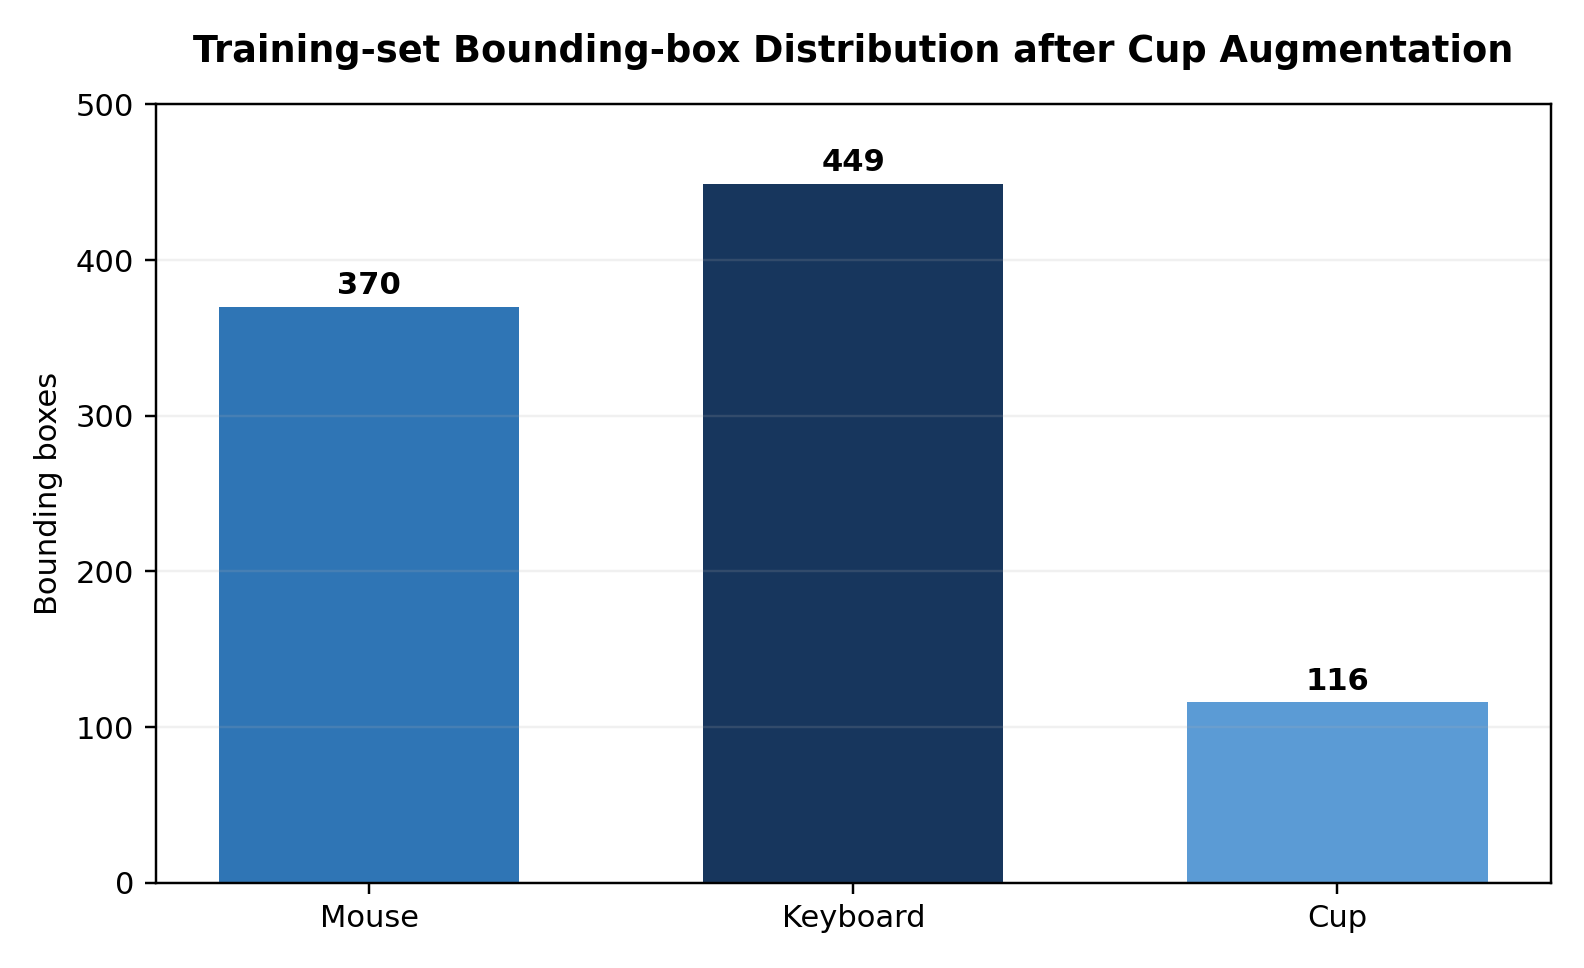
\includegraphics[width=\linewidth]{figures/dataset-class-distribution.png}\caption{Bounding-box distribution}\end{subfigure}\hfill
\begin{subfigure}[t]{0.55\textwidth}\centering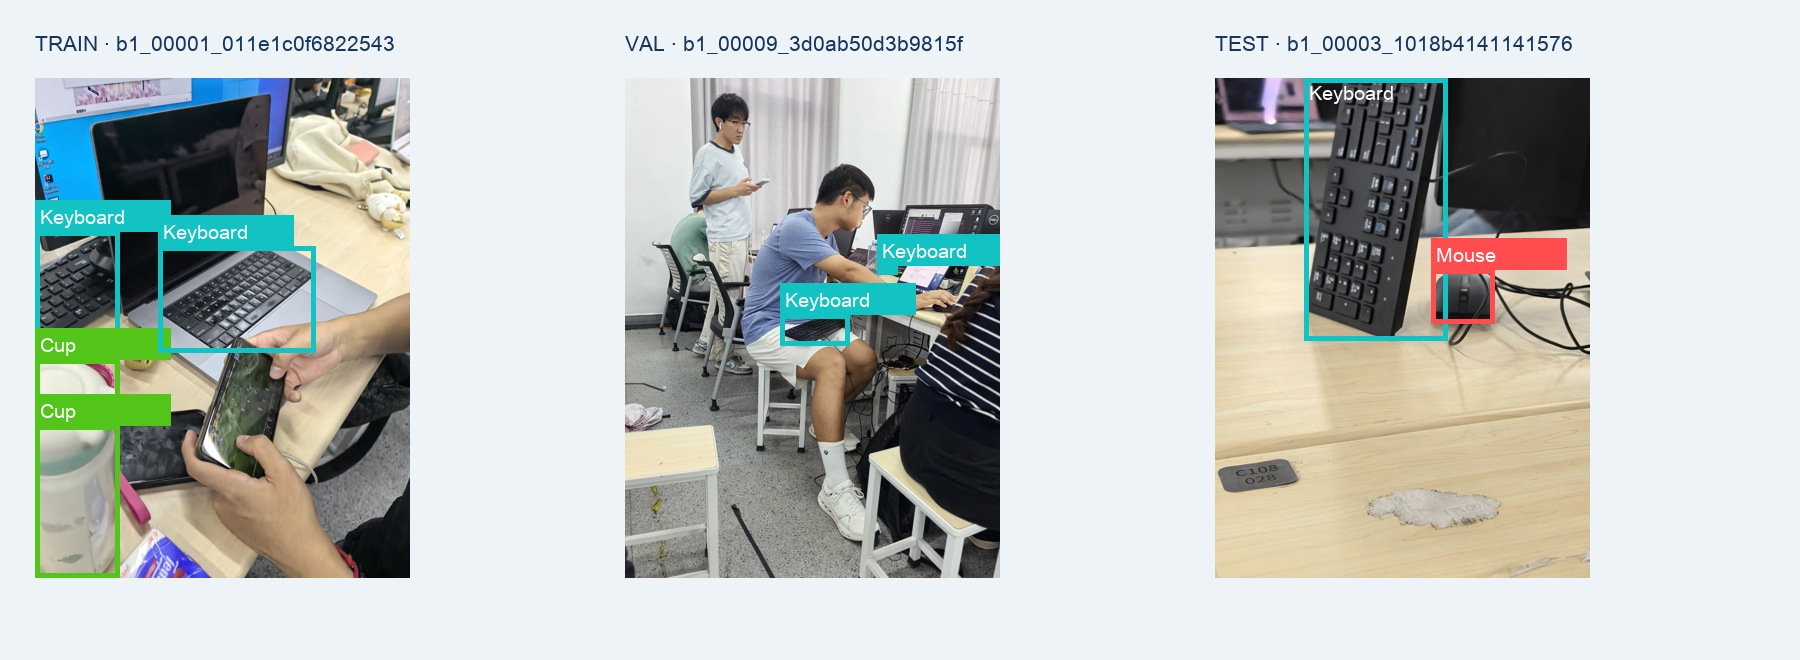
\includegraphics[width=\linewidth]{figures/dataset-annotation-montage.jpg}\caption{YOLO labels rendered on audited images}\end{subfigure}
\caption{Dataset statistics and annotation evidence generated from the audited subset}\label{fig:data}
\end{figure}

\subsection{Near-duplicate control and data leakage prevention}
Desktop images are frequently captured in bursts or extracted from video, so adjacent frames can be almost identical in background, illumination, and object position. A purely random image-level split may place such frames in both training and test sets and produce overly optimistic metrics. Samples were therefore grouped by capture batch, video segment, and consecutive filename range before splitting. The augmented Cup samples inherit the training-only status of their sources. Perceptual hashing can be added as a second screening step, and the test set must remain untouched while augmentation parameters and confidence thresholds are selected.

\subsection{Annotation governance and data provenance}
Each image should be traceable to a source category, capture batch, review state, split membership, and annotation revision. A compact manifest can record these fields together with a file hash, enabling duplicate detection and preventing an online image, augmented derivative, or corrected label from silently changing partitions. Online material must also retain its source URL and license status outside the public dataset archive. This governance separates original evidence from derived training data and makes later corrections auditable without committing large image files to GitHub.

\section{YOLOv8 Model Training}
YOLOv8n was selected as the edge baseline because of its small parameter count and low latency. Training started from general pretrained weights with an input size of $640\times640$, batch size 8, and 100 epochs on MPS. The objective combines box regression, classification, and distribution focal loss:
\begin{equation}\mathcal{L}=\lambda_{box}\mathcal{L}_{box}+\lambda_{cls}\mathcal{L}_{cls}+\lambda_{dfl}\mathcal{L}_{dfl}.\end{equation}
Brightness and saturation perturbation, scale, translation, horizontal flipping, and Mosaic augmentation improve generalization when their parameters are validated rather than maximized. Strong unrealistic rotations are avoided for keyboards with directional layouts.

For evaluation,
\begin{equation}P=\frac{TP}{TP+FP},\qquad R=\frac{TP}{TP+FN}.\end{equation}
AP is the area under the precision-recall curve, while mAP averages AP across classes. Both mAP@0.5 and mAP@0.5:0.95 are reported to avoid overestimating localization quality at a single IoU threshold.

YOLOv8s may be evaluated under the same split, image size, epochs, and test procedure. It should replace YOLOv8n only if its accuracy gain justifies the additional latency and it remains above 5 FPS on Jetson. This is a planned controlled comparison, not a claimed completed result.

\begin{table}[htbp]\centering\caption{Edge-model comparison and selection criteria}
\begin{tabularx}{0.9\textwidth}{lXXX}\toprule
\textbf{Model} & \textbf{Main advantage} & \textbf{Main cost} & \textbf{Selection condition}\\\midrule
YOLOv8n & Low parameter count and latency & Lower potential accuracy ceiling & Real-time performance or limited compute is the priority\\
YOLOv8s & Stronger feature representation & Higher latency and memory use & Measured Jetson speed remains above 5 FPS\\\bottomrule
\end{tabularx}\end{table}

The comparison must use the same random seed and report parameter count, serialized model size, per-class AP, peak memory, mean FPS, minimum FPS, and end-to-end latency. This prevents an apparent accuracy gain from being caused by a different split or a more favorable threshold.

\section{Training and Validation Results}
\begin{table}[htbp]\centering\caption{YOLOv8n validation results}\label{tab:metrics}
\begin{tabular}{lccl}\toprule \textbf{Metric} & \textbf{Value} & \textbf{Assessment} & \textbf{Interpretation}\\\midrule
Precision & 0.806 & High & Relatively few false positives\\
Recall & 0.894 & High & Relatively few missed targets\\
mAP@0.5 & 0.888 & Good & Strong performance at IoU 0.5\\
mAP@0.5:0.95 & 0.814 & Good & Robust localization under stricter IoU\\\bottomrule
\end{tabular}\end{table}

The recorded Mac timings were 1.3 ms for preprocessing, 27.7 ms for network inference, and 10.3 ms for postprocessing, giving
\begin{equation}\mathrm{FPS}\approx\frac{1000}{1.3+27.7+10.3}=25.45.\end{equation}
This is a host-side value and does not replace end-to-end Jetson measurement, which includes capture, rendering, and scheduling overhead.

\begin{figure}[htbp]\centering
\begin{subfigure}[t]{0.32\textwidth}\centering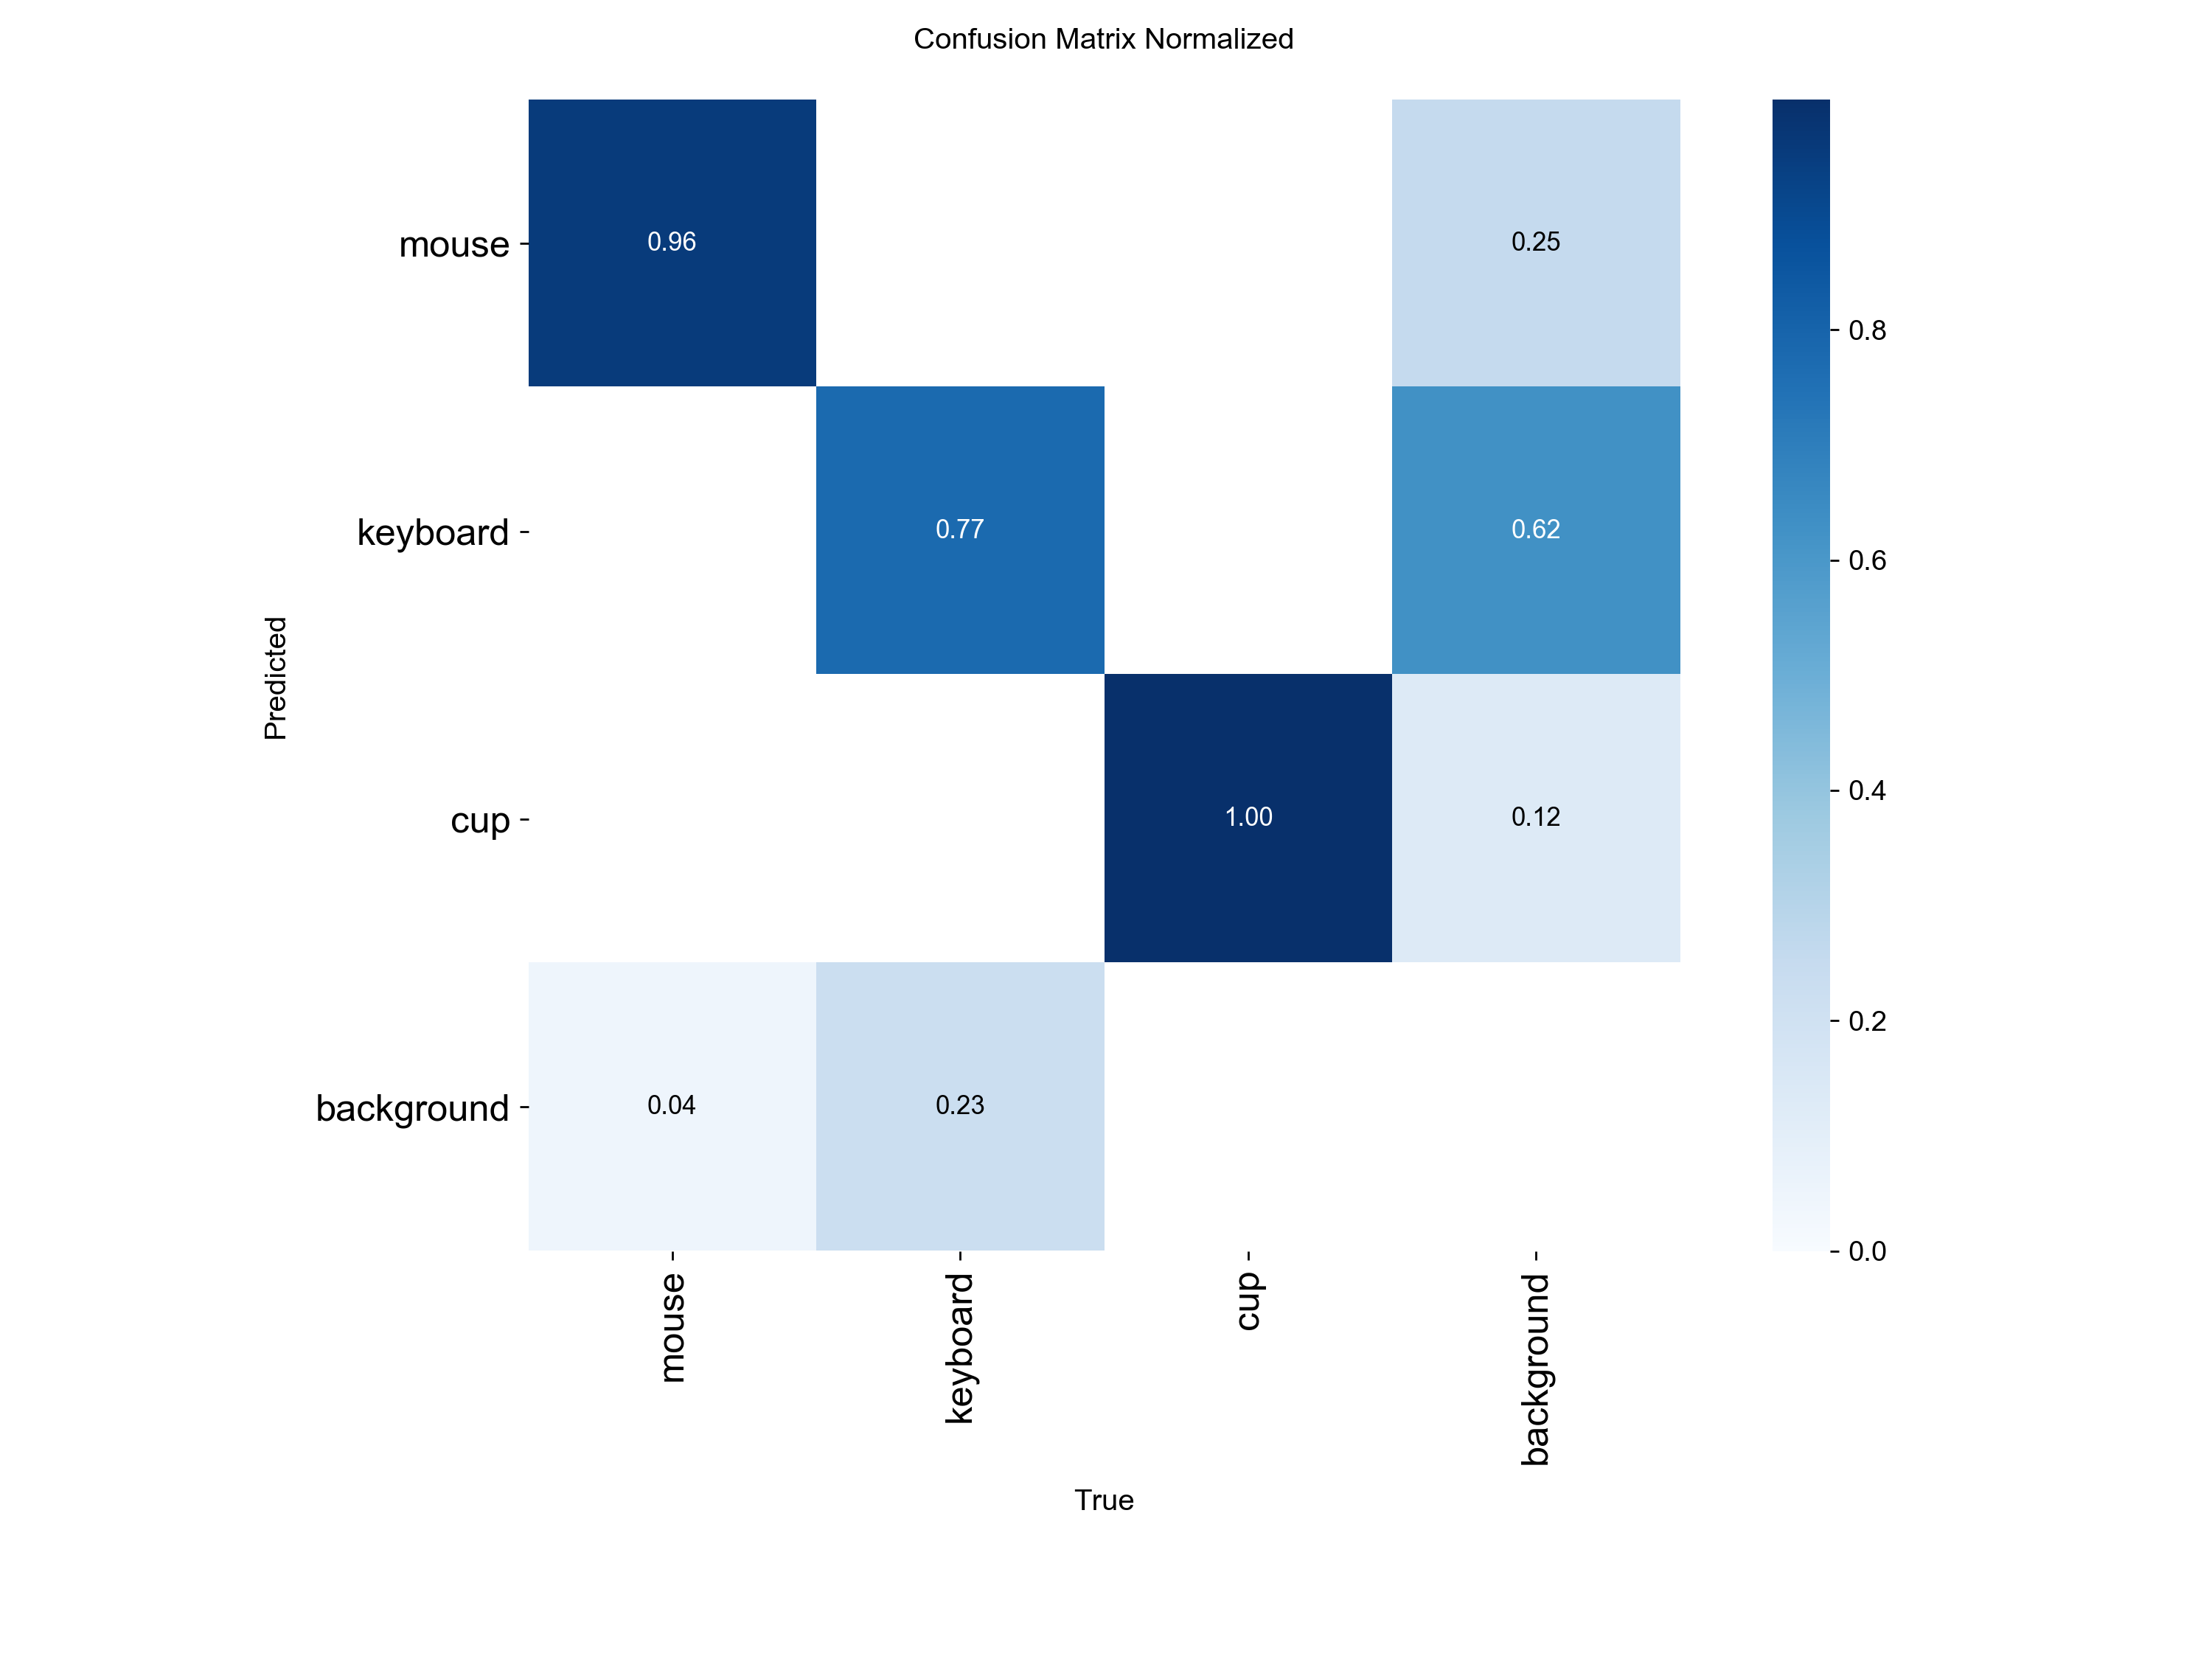
\includegraphics[width=\linewidth]{figures/confusion-matrix-normalized.png}\caption{Normalized confusion matrix}\end{subfigure}\hfill
\begin{subfigure}[t]{0.32\textwidth}\centering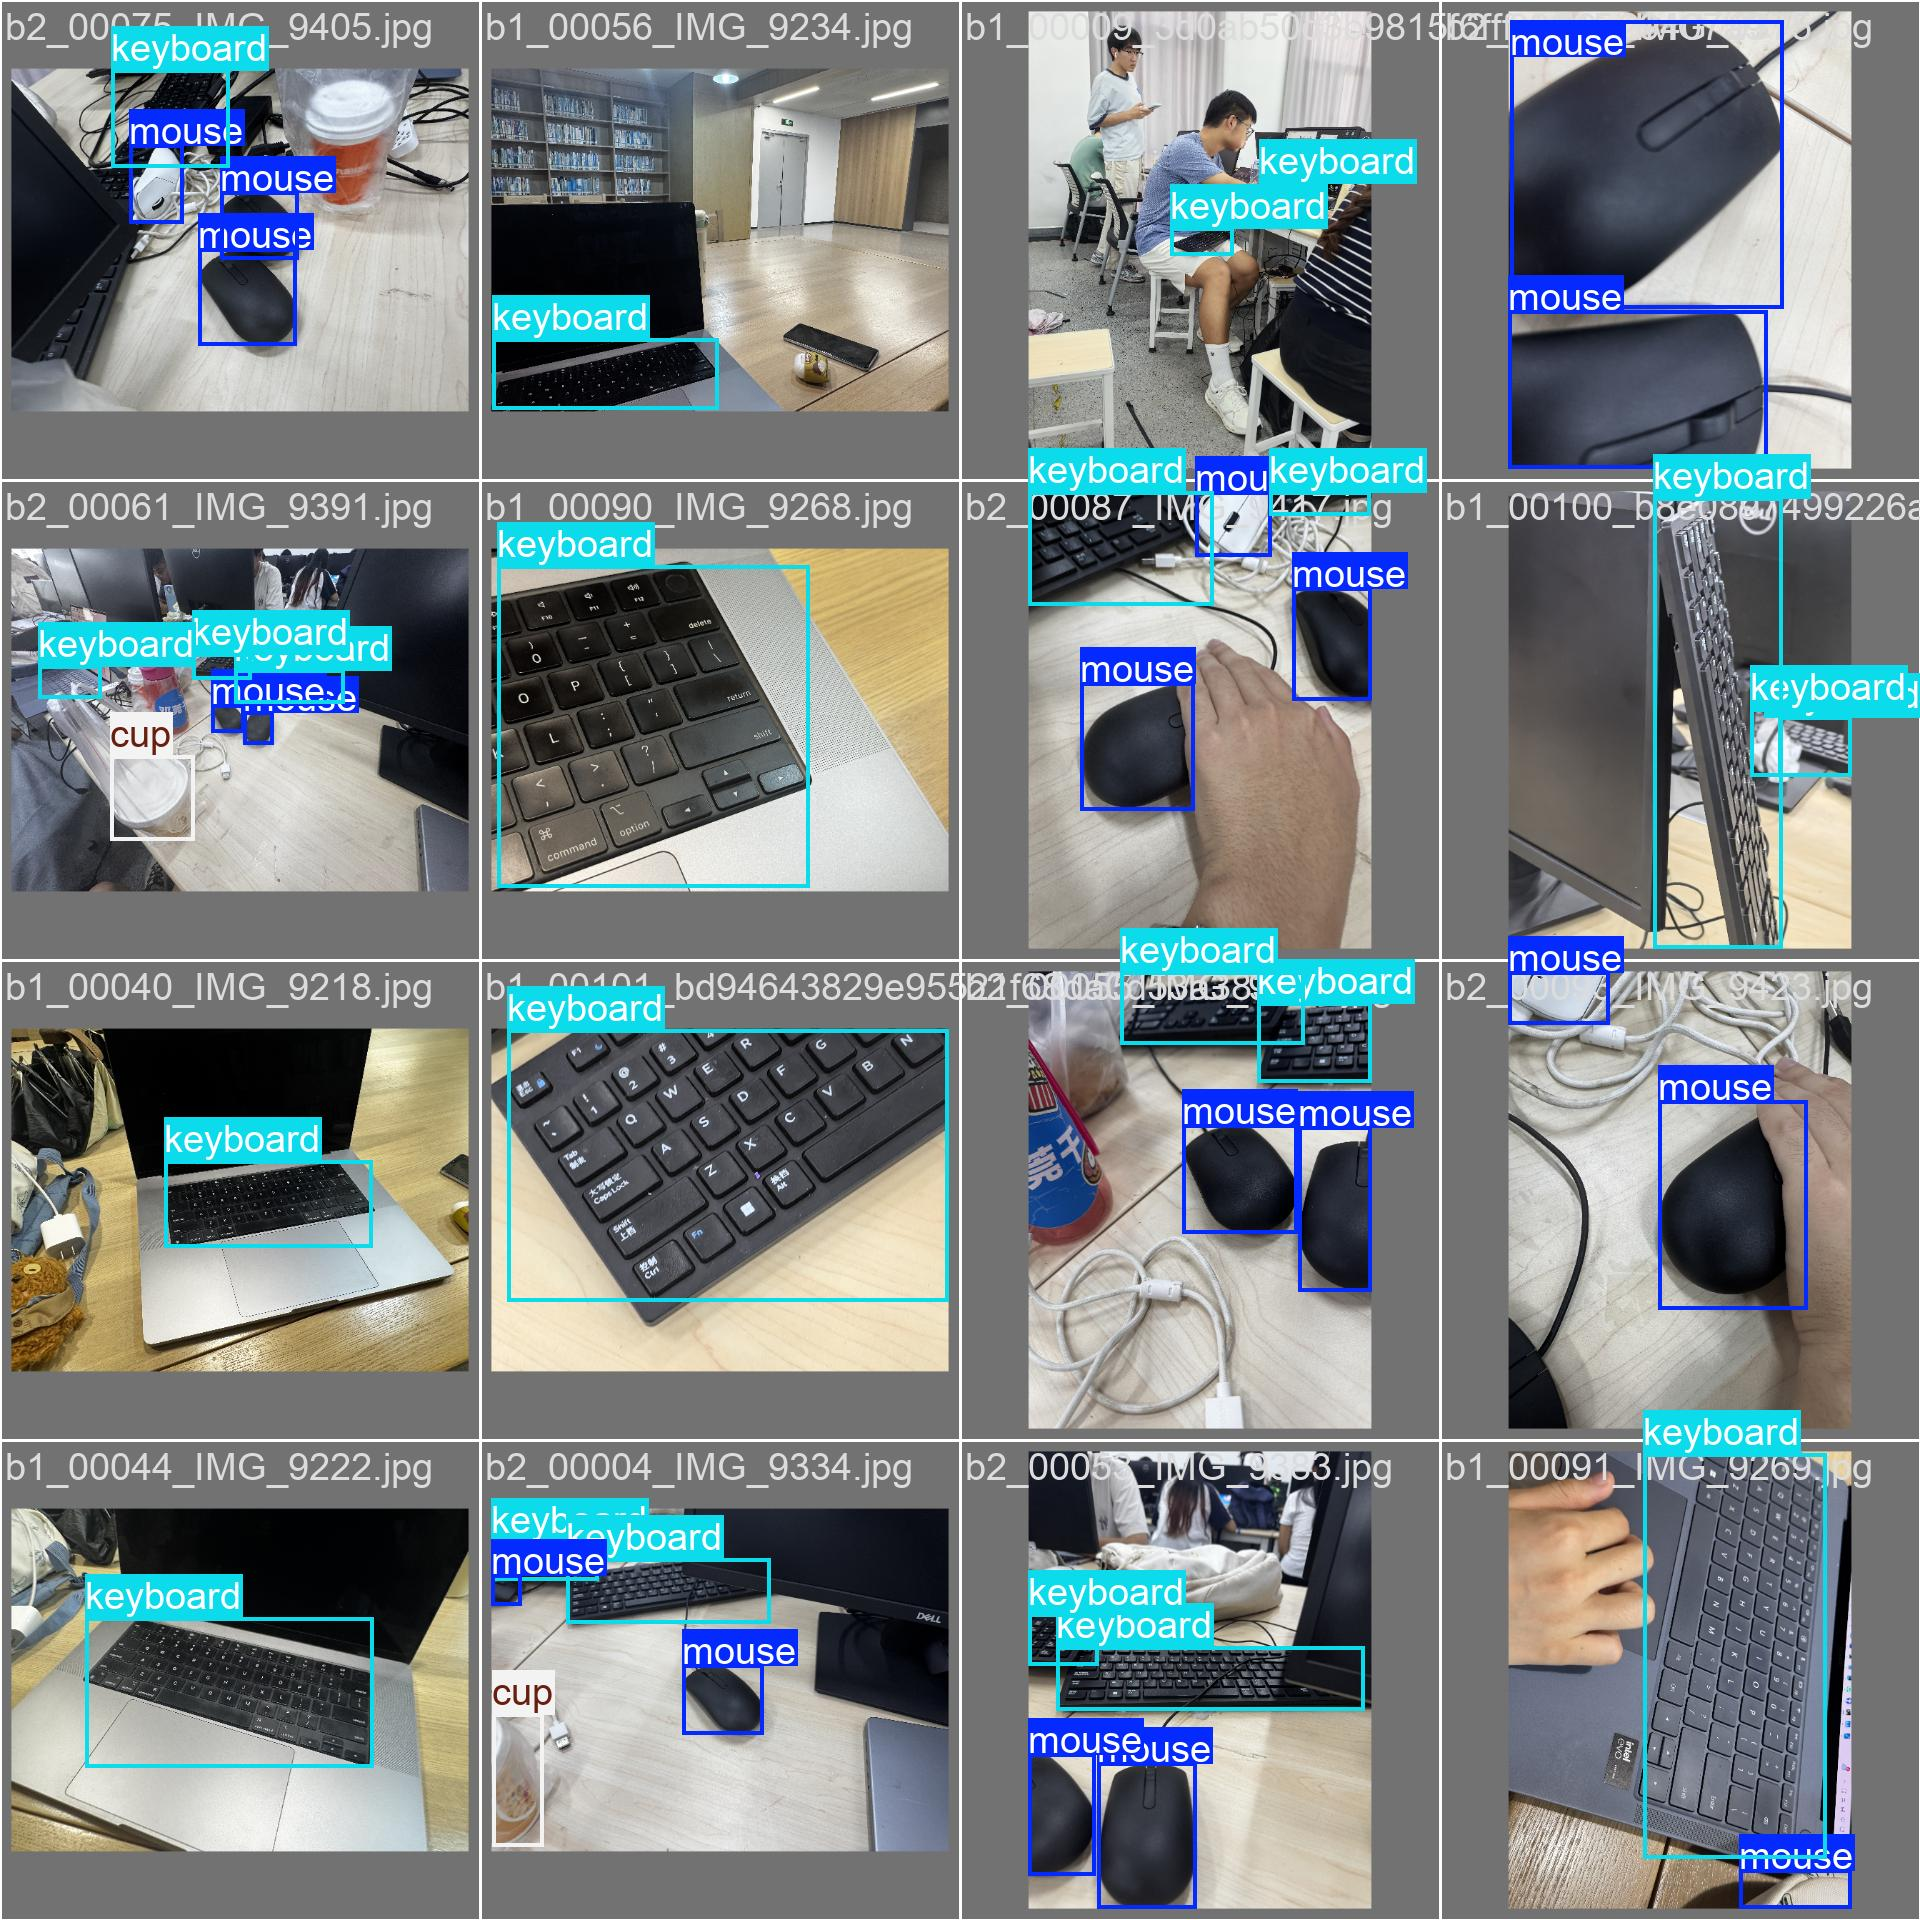
\includegraphics[width=\linewidth]{figures/val-labels.jpg}\caption{Validation labels}\end{subfigure}\hfill
\begin{subfigure}[t]{0.32\textwidth}\centering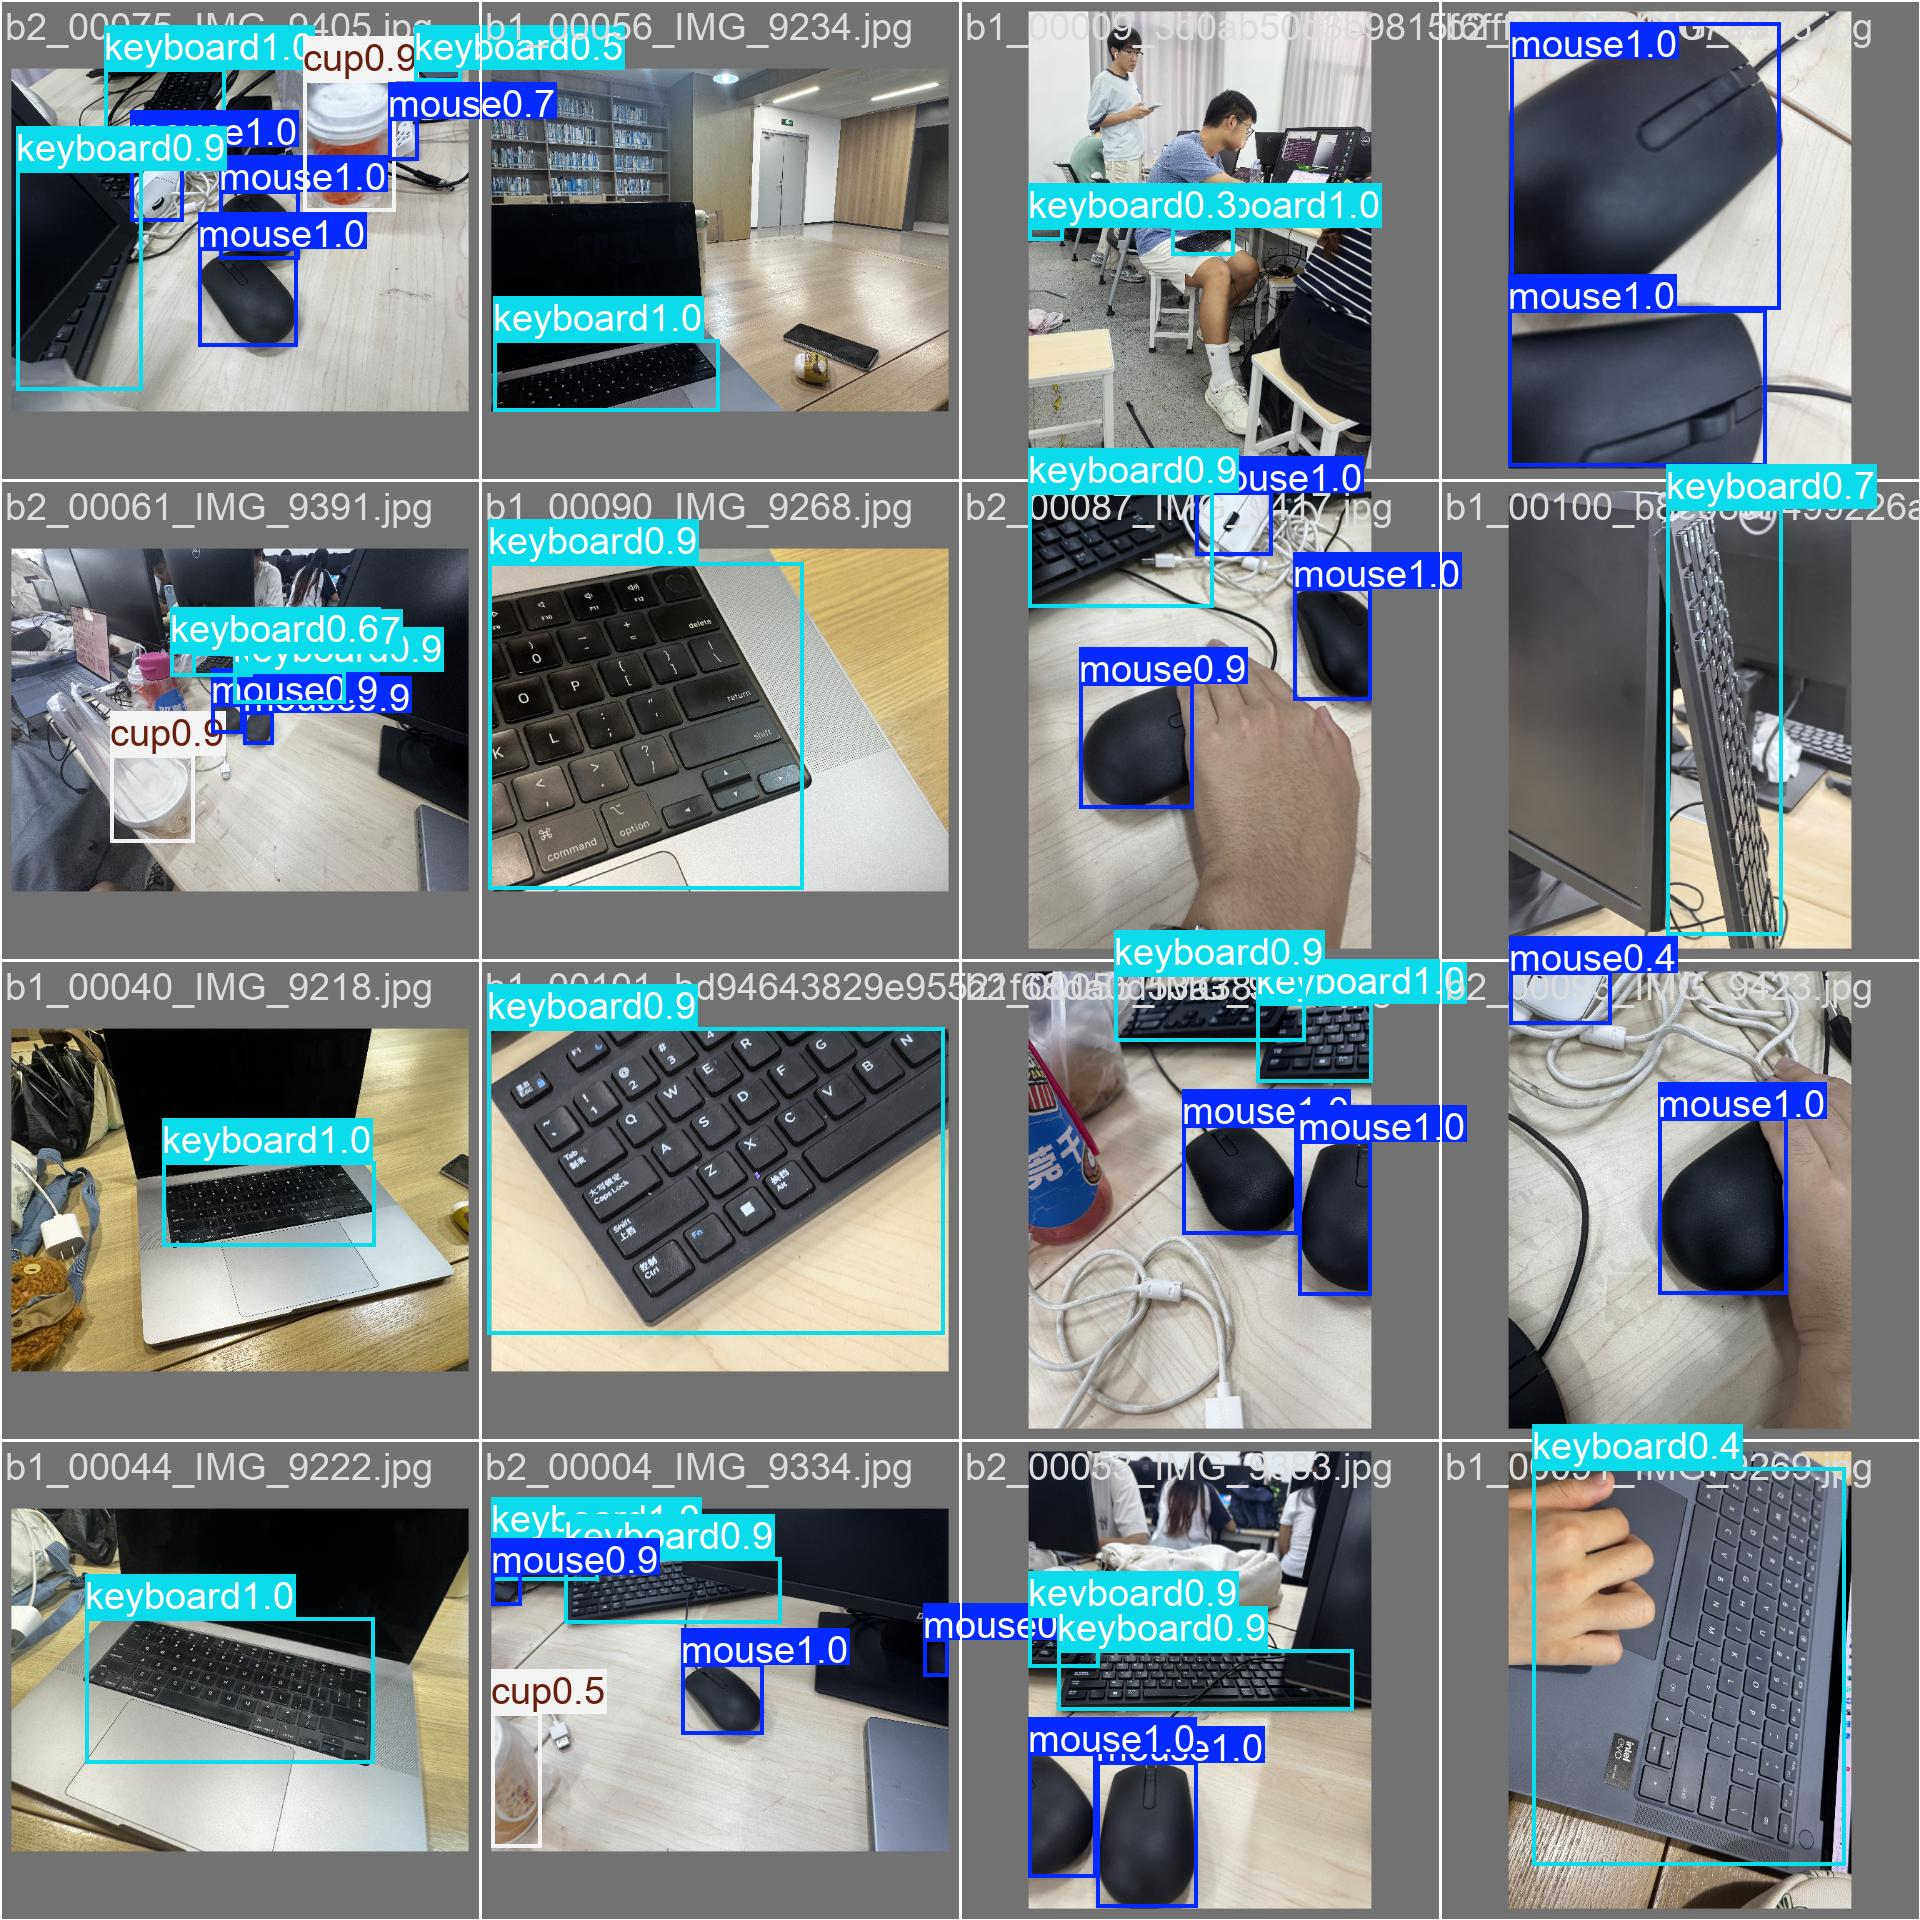
\includegraphics[width=\linewidth]{figures/val-pred.jpg}\caption{Validation predictions}\end{subfigure}
\caption{Validation and error-analysis evidence retained by the training pipeline}\label{fig:validation}
\end{figure}

Mouse and Keyboard have more training instances and more stable outlines. Cup is less frequent and varies substantially because of transparency, reflection, handles, and background color. Confidence thresholds therefore require class-aware review: lowering the threshold improves recall but introduces more false positives, whereas raising it can suppress small or occluded targets.

\subsection{Ablation protocol}
An ablation study should isolate the contribution of each data-engineering decision. The baseline uses the audited source set with default augmentation. Subsequent runs add Cup-focused offline augmentation, negative backgrounds, and deployment hard cases one factor at a time. Model architecture, epoch count, image size, split, and evaluation script remain fixed. Overall metrics must be reported together with Cup recall and the number of background false positives.

\begin{table}[htbp]\centering\caption{Controlled ablation plan}
\begin{tabularx}{0.92\textwidth}{lXX}\toprule
\textbf{Run} & \textbf{Single controlled change} & \textbf{Expected evidence}\\\midrule
A & Audited source set only & Reproducible baseline\\
B & Add Cup-focused augmentation & Improved Cup recall and robustness\\
C & Add negative backgrounds & Fewer desk-edge and package false positives\\
D & Add deployment hard cases & Better low-light, occlusion, and small-object behavior\\\bottomrule
\end{tabularx}\end{table}

\begin{figure}[htbp]\centering
\begin{subfigure}[t]{0.49\textwidth}\centering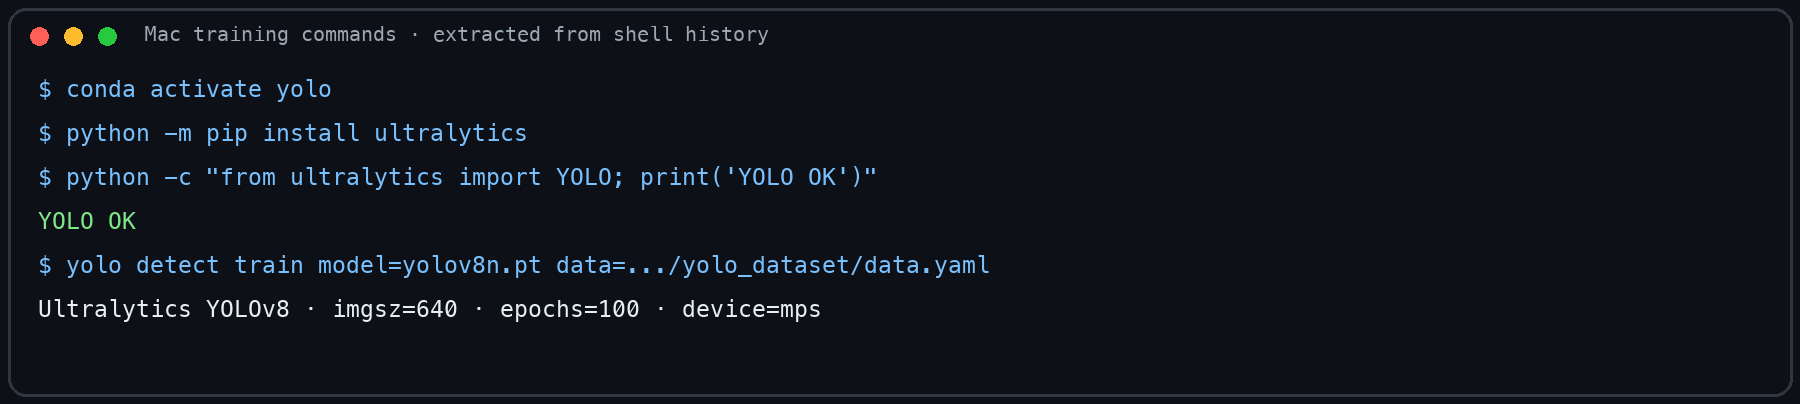
\includegraphics[width=\linewidth]{figures/training-command-history.png}\caption{Training commands recorded on the Mac}\end{subfigure}\hfill
\begin{subfigure}[t]{0.49\textwidth}\centering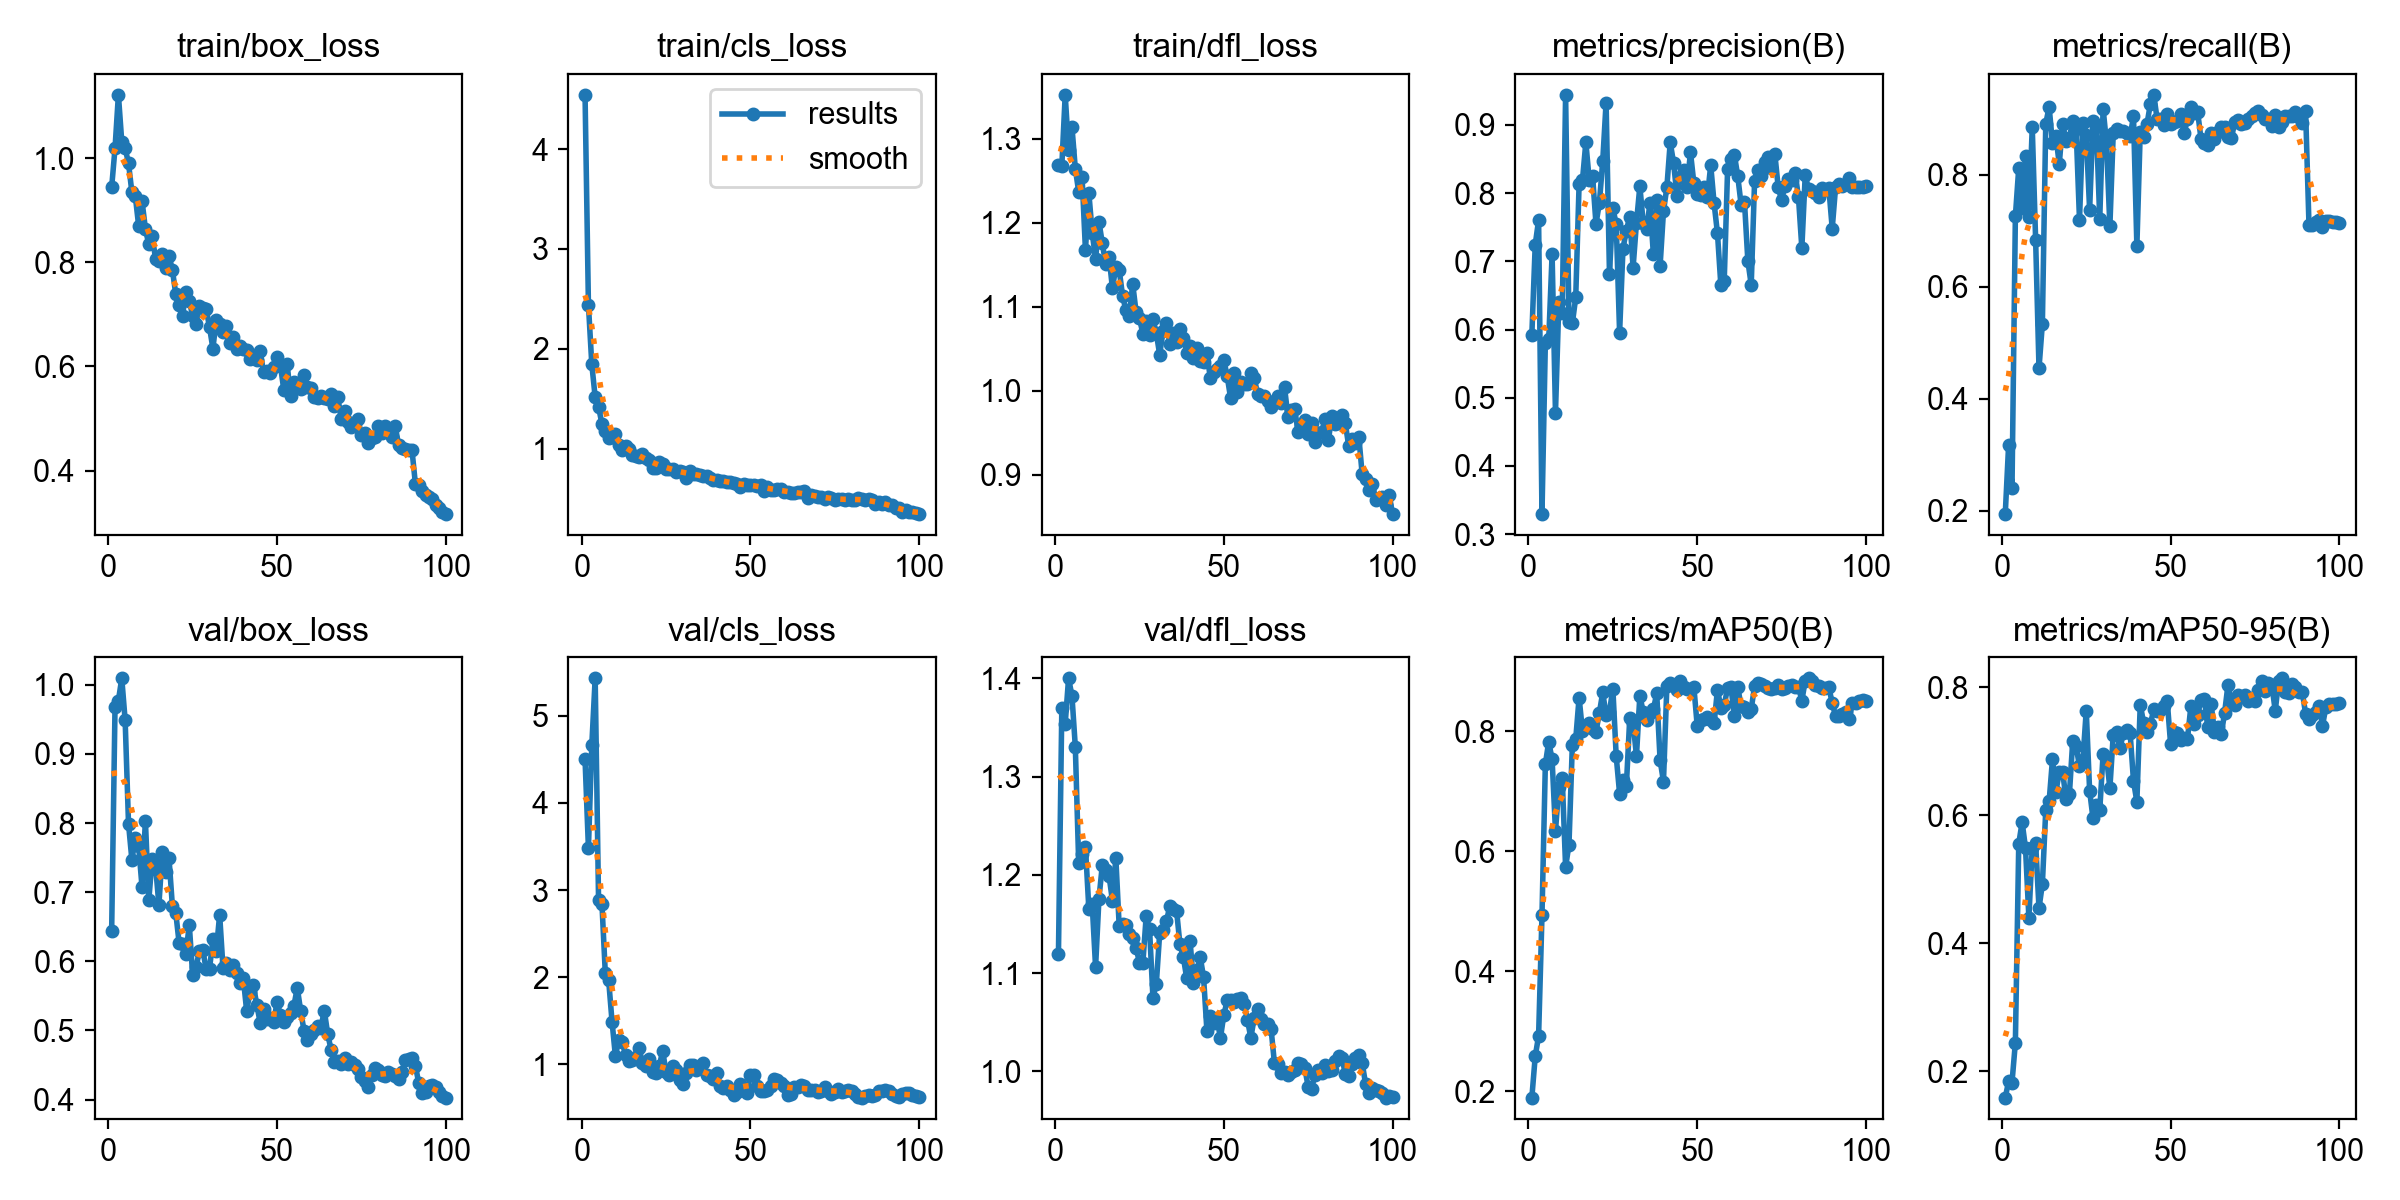
\includegraphics[width=\linewidth]{figures/training-results.png}\caption{Metrics over 100 epochs}\end{subfigure}
\caption{Training execution and convergence evidence}\label{fig:training}
\end{figure}

\section{Jetson Deployment and Runtime Results}\label{sec:jetson}
The trained \texttt{best.pt} model was transferred to Jetson. OpenCV captures each frame, YOLOv8 returns class identifiers, confidence scores, and bounding boxes, and the program draws the results while measuring FPS. The program can save video and CSV logs and can publish the same structured output for downstream perception or control nodes.

Training and deployment are deliberately decoupled. The Mac performs dataset processing, accelerated training, and offline evaluation, whereas the Jetson performs capture, inference, rendering, logging, and communication. Versioned weights make rollback possible when a newer model improves offline mAP but behaves less reliably under the live camera domain. Runtime logging records timestamps, classes, confidence values, pixel coordinates, and frame rate so that failures can be traced back to exact frames.

TensorRT FP16 export is a reproducible optimization path that can reduce compute and memory use. A valid comparison must keep image resolution, confidence threshold, camera input, and power mode fixed and report pure inference latency, end-to-end latency, mean and minimum FPS, and memory usage. TensorRT acceleration is not presented here as a completed measurement.

Container metadata reports a 1280$\times$720 video, 300 frames, 20.0 s duration, and a nominal rate of 15 FPS. Manual inspection at the beginning, middle, and later portions shows an overlay between 14.8 and 15.0 FPS. The video demonstrates Keyboard, Mouse, and Cup across the sequence; it does not constitute a frame-by-frame accuracy test. Visible examples include Mouse confidence 0.93 near the beginning and Cup confidence around 0.91--0.93 after it enters the scene. Figure~\ref{fig:jetson} shows representative multi-object frames.

\begin{figure}[htbp]\centering
\begin{subfigure}[t]{0.485\textwidth}\centering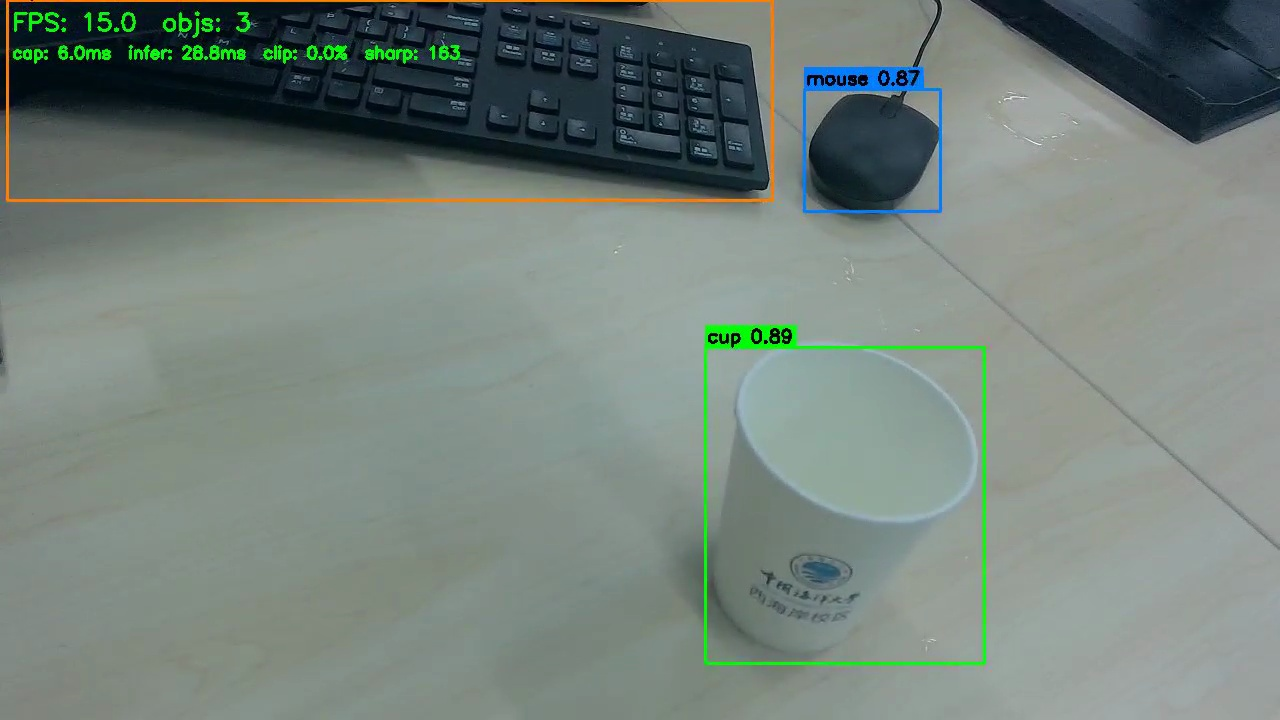
\includegraphics[width=\linewidth]{figures/jetson-cup.jpg}\caption{Three classes detected; Cup confidence 0.89}\end{subfigure}\hfill
\begin{subfigure}[t]{0.485\textwidth}\centering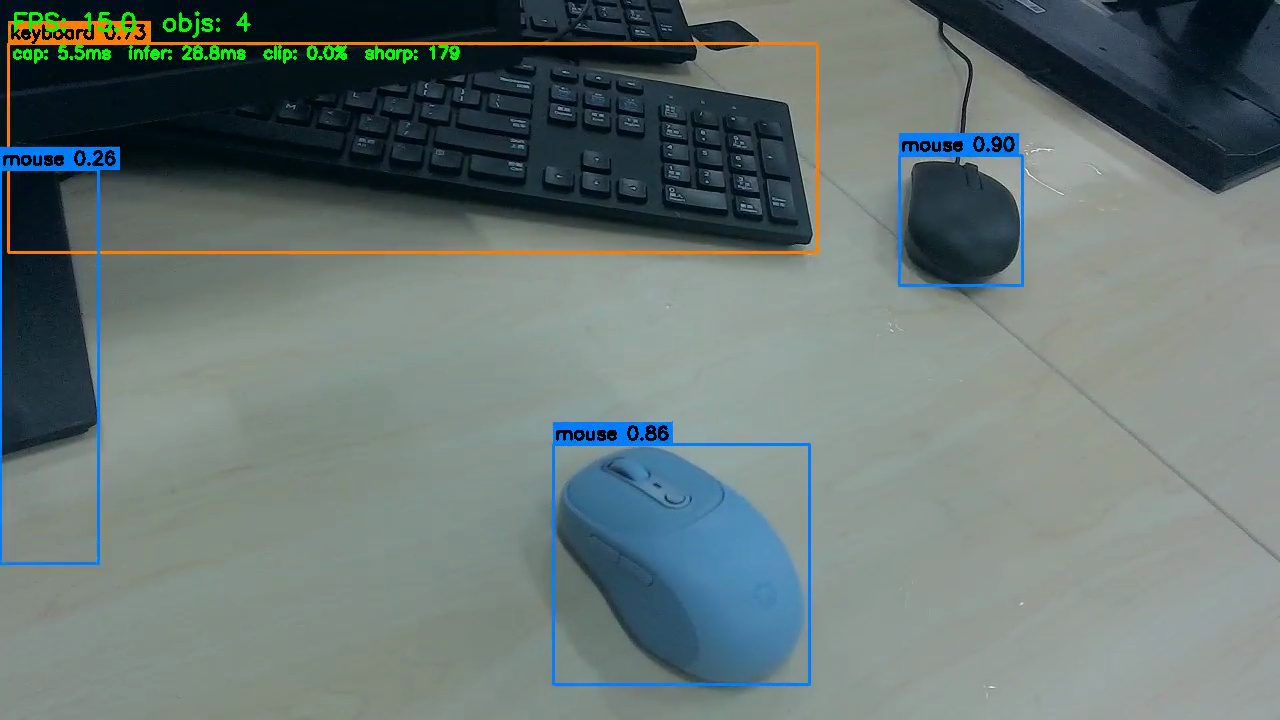
\includegraphics[width=\linewidth]{figures/jetson-multiobject.jpg}\caption{Keyboard and multiple mice detected}\end{subfigure}
\caption{Real-time Jetson camera detections extracted from the final video}\label{fig:jetson}\end{figure}

\begin{table}[htbp]\centering\caption{Measured results from the final Jetson video}
\begin{tabular}{ll}\toprule \textbf{Test item} & \textbf{Measured result}\\\midrule
Video specification & 1280$\times$720, 300 frames\\
Duration and frame rate & 20.0 s; nominal 15 FPS, observed overlay 14.8--15.0 FPS\\
Representative inference time & 28.8 ms\\
Representative image-processing time & 6.0 ms\\
Detected classes & Keyboard, Mouse, Cup\\
Real-time requirement & Lowest inspected overlay 14.8 FPS $>$ 5 FPS\\\bottomrule
\end{tabular}\end{table}

\subsection{ROS2 interface and offline verification}
The deployment program implements an \texttt{rclpy} node named \texttt{desk\_object\_detector}. It publishes JSON through \texttt{std\_msgs/String} on \texttt{/desk\_object\_detections}. Each payload contains the frame index, timestamp, FPS, class identifier, class name, confidence, and pixel coordinates $[x_1,y_1,x_2,y_2]$.

ROS2, \texttt{colcon}, and \texttt{rclpy} were not installed on the Mac. Consequently, the evidence below is an actual serialization, deserialization, and schema check of the same payload, not a fabricated \texttt{ros2 topic echo}. Live topic echo remains to be verified in the Jetson ROS2 environment.

\begin{figure}[htbp]\centering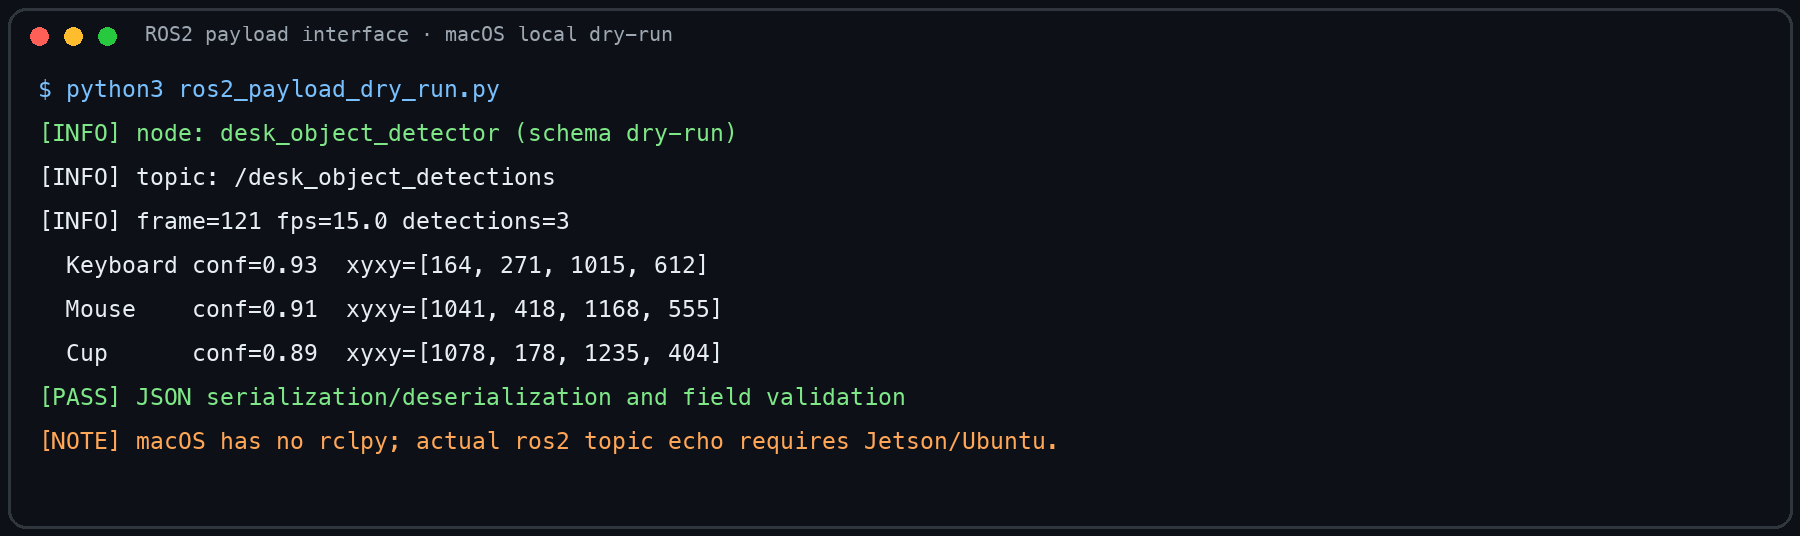
\includegraphics[width=0.88\textwidth]{figures/ros2-payload-dry-run.png}
\caption{Offline validation of the ROS2 message payload on Mac (not a live topic echo)}\label{fig:ros}
\end{figure}

For the required 20-object acceptance test, at least 20 physical instances should cover the three classes, viewpoints, distances, and occlusion levels. Each correct detection, missed detection, and false detection must be recorded. The acceptance accuracy is the number of correctly recognized objects divided by the total number tested. This result must be reported separately from mAP.

System-level evaluation should additionally report average and minimum FPS, preprocessing, inference, and postprocessing latency, message publication frequency, dropped frames, and continuous-run stability. These measures distinguish model accuracy from the behavior of the complete camera-to-message pipeline.

\section{Error Analysis and Improvements}
The video contains short, credible failure cases rather than perfectly stable detections. Around the 7 s region, the overlay reports four objects although the scene principally contains one keyboard, one mouse, and one cup; an additional Keyboard box with confidence 0.43 extends over the right-hand desk/hand region. Around 15 s, a hand-held black mouse is assigned a low-confidence Mouse detection of 0.32, but the box expands over much of the hand and arm. These observations show that the model is sensitive to occlusion, hand--object interaction, and elongated high-contrast background structures. They are qualitative video observations, not a counted error rate.

A practical correction strategy is to add empty desk regions, hands, forearms, monitor bases, cables, and partial keyboard edges as hard negatives, while adding manually reviewed hand-held Mouse examples as hard positives. Confidence-threshold tuning alone would suppress the 0.43 false Keyboard box but could also remove the valid 0.32 occluded Mouse detection. The preferred remedy is therefore targeted hard-case retraining followed by evaluation on the unchanged test set.

Domain shift also exists between training images and Jetson video because of focal length, exposure, motion blur, and viewpoint. Cup is especially vulnerable under reflections, low light, and background-color similarity. Error frames should be categorized as low light, occlusion, small object, clutter, or motion blur, manually reviewed, and added to the next training round. A controlled ablation can then compare the baseline, augmentation, negative samples, and hard-case feedback while keeping the split and training settings fixed.

\section{Engineering Contributions}
\subsection{Human-in-the-loop annotation}
Automatic pre-annotation followed by manual review provides an efficient and reliable dataset workflow. Candidate boxes reduce repetitive drawing effort, while human decisions remain responsible for class correctness, missed objects, tight boundaries, and difficult Cup instances. The workflow can be repeated when new classes or deployment scenes are introduced.

\subsection{Dataset quality as an engineering task}
The project goes beyond reporting only image and box counts. It checks orphan labels, invalid classes, out-of-range coordinates, empty labels, imbalance, and near duplicates, then uses grouped splitting to limit leakage. The detection and isolation of 15 abnormal labels is a directly verifiable outcome of this audit. Cup-focused augmentation further addresses imbalance using real verified boxes rather than fabricated counts.

\subsection{From a model demo to an edge perception system}
Camera input, YOLO inference, overlays, frame-rate measurement, saved evidence, and a ROS2-compatible output are integrated into one deployment path. YOLOv8n camera inference has been measured, while YOLOv8s comparison and TensorRT FP16 remain explicitly identified as future controlled optimizations rather than completed results.

\subsection{Error-driven closed-loop improvement}
The deployment domain differs from still training images in focal length, exposure, blur, and viewpoint. Saving low-confidence and incorrect frames converts runtime behavior into traceable data tasks. After categorization and manual review, those samples can be added to training and compared on the fixed test set. This loop is more informative than increasing epochs without diagnosing the source of error.

\section{Project Archive and Reproducibility}
Code, dataset configuration, audited labels, the trained model, training results, and the report are organized in the personal repository \href{https://github.com/Gabriel6002/-1}{Gabriel6002/-1}. Large image collections and the final video are intentionally excluded from GitHub. The repository uses one clear location for each artifact category: \texttt{scripts/}, \texttt{data/}, \texttt{models/}, \texttt{results/}, \texttt{report/}, and \texttt{docs/}.

For deployment repeatability, the model file, class order, input resolution, confidence threshold, software versions, and Git revision should be logged together. Timing measurements should include a warm-up period and distinguish pure model inference from camera decoding, preprocessing, drawing, ROS2 serialization, and video writing. Recording mean, minimum, and percentile latency avoids presenting a single favorable frame as system performance.

\begin{table}[htbp]\centering\caption{Reproducibility checklist and evidence boundary}\label{tab:repro}
{\renewcommand{\arraystretch}{1.08}\begin{tabular}{p{4.4cm}p{5.1cm}p{4.0cm}}\toprule
\textbf{Artifact or check} & \textbf{Repository evidence} & \textbf{Status}\\\midrule
Training and dataset code & \texttt{scripts/}, \texttt{data/data.yaml} & Archived and syntax-checked\\
Audited annotations & \texttt{data/labels/} & 270 files, 935 valid boxes\\
Trained detector & \texttt{models/best.pt} & Archived, non-empty file\\
Learning evidence & \texttt{results/training/} & Metrics and plots archived\\
Jetson demonstration & Video retained outside GitHub & 15 FPS display observed\\
ROS2 payload & Publisher code and offline JSON check & Live topic echo not claimed\\
Raw images and video & Excluded by repository policy & Kept outside public Git history\\\bottomrule
\end{tabular}}\end{table}

\subsection{Validity boundaries}
The 45 Cup augmentations increase training exposure but are correlated derivatives, not independent test evidence; consequently, they are excluded from validation and testing. The approximately 650-image integrated pool combines self-collected, online, and negative material, whereas the 225-image core is the subset with complete audited image--label correspondence. Domain shift can remain between online imagery and the Jetson camera. Finally, the ROS2 message structure has been validated offline, but a live Jetson \texttt{ros2 topic echo} result is not presented. These boundaries distinguish measured results from engineering proposals.

\begin{center}\vspace{-0.4em}
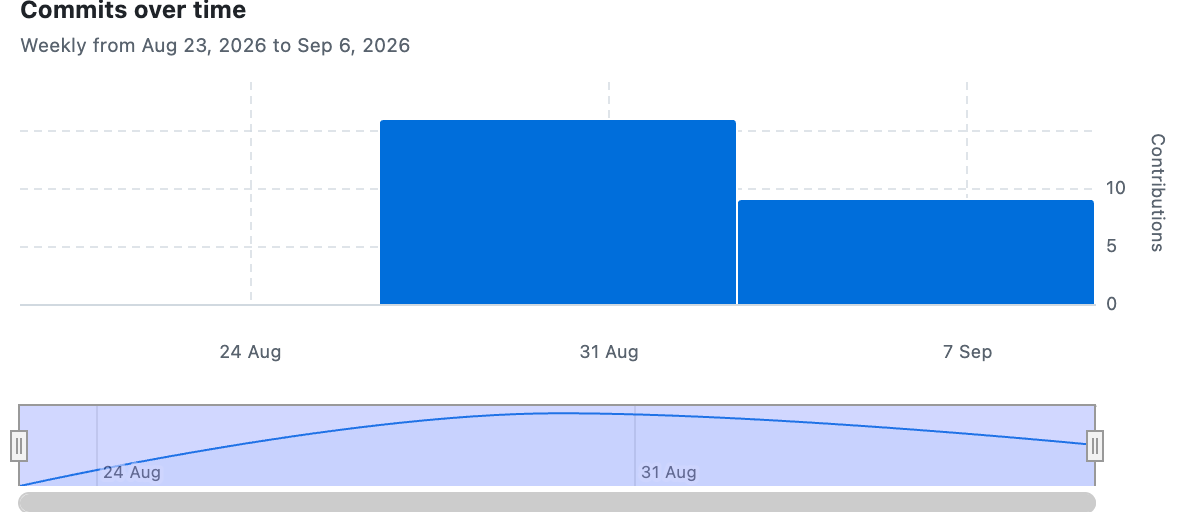
\includegraphics[width=0.80\textwidth]{figures/github-commit-history.png}
\captionof{figure}{Incremental Git commit history generated from the local repository log}\label{fig:git}
\vspace{-0.5em}\end{center}

\section{Conclusion}
This experiment completed an end-to-end desktop object detector from multi-source dataset construction to real-time Jetson execution. The integrated dataset contains approximately 650 source images, including self-collected positives, supplementary online samples, and negative backgrounds. The audited core contains 225 source images and 687 positive boxes, and quality control prevented 15 orphan labels from entering training. A further 45 training-only augmented samples increased the training representation to 935 boxes, including 116 Cup instances. YOLOv8n achieved precision 0.806, recall 0.894, mAP@0.5 0.888, and mAP@0.5:0.95 0.814. The 20 s video includes detections of Keyboard, Mouse, and Cup and shows approximately 14.8--15.0 FPS in inspected frames, satisfying the 5 FPS requirement. It also preserves transient failure cases that motivate hard-negative and occlusion-focused refinement.

The work shows that a complete object-detection experiment requires dataset quality control, independent evaluation, hardware deployment, latency measurement, reproducible archiving, and error feedback. Future work should collect additional independent Cup scenes, continue expanding hard negative samples, and complete live ROS2 topic verification on Jetson.

\clearpage
\section*{References}\addcontentsline{toc}{section}{References}
\begin{enumerate}[label={\lbrack\arabic*\rbrack},leftmargin=2.6em,nosep]\small
\item G. Jocher, A. Chaurasia, and J. Qiu, ``Ultralytics YOLO,'' 2023. [Online]. Available: \url{https://github.com/ultralytics/ultralytics}
\item J. Redmon, S. Divvala, R. Girshick, and A. Farhadi, ``You Only Look Once: Unified, Real-Time Object Detection,'' in \emph{Proc. CVPR}, 2016, pp. 779--788.
\item NVIDIA, ``NVIDIA TensorRT Developer Guide.'' [Online]. Available: \url{https://docs.nvidia.com/deeplearning/tensorrt/}
\item Open Robotics, ``ROS 2 Documentation.'' [Online]. Available: \url{https://docs.ros.org/}
\item\label{openimages} A. Kuznetsova et al., ``The Open Images Dataset V4: Unified Image Classification, Object Detection, and Visual Relationship Detection at Scale,'' \emph{Int. J. Comput. Vis.}, vol. 128, pp. 1956--1981, 2020. Dataset: \url{https://storage.googleapis.com/openimages/web/index.html}
\end{enumerate}
\end{document}
